\begin{frame}
 \frametitle{C and C++ - Executables and Address Spaces}
 \begin{itemize}
  \item executables consist of shareable sections
   \begin{description}
    \item[\binarycode{.text}] program code
    \item[\binarycode{.rodata}] read-only data
   \end{description}
  \item and non-shareable sections
   \begin{description}
    \item[\binarycode{.data}] write-able data
    \item[\binarycode{.bss}] zero-initialized writeable data
   \end{description}
 \end{itemize}

 \begin{figure}
  \centering {
   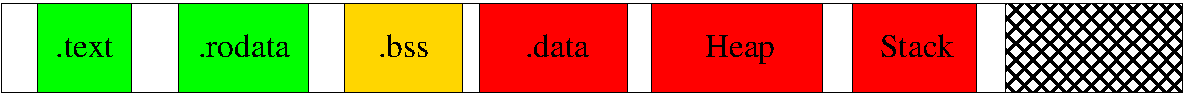
\includegraphics[scale=0.5]{layout-eps.pdf}
  }
  \caption{Memory layout}
 \end{figure}

 \begin{itemize}
  \item address spaces are composed of executable's sections plus
   \begin{itemize}
    \item stack
    \item heap memory
   \end{itemize}
 \end{itemize}
\end{frame}

\begin{frame}
 \frametitle{C and C++ - Static Memory Allocation}
 \begin{itemize}
  \item static data will be stored in binary
  \item maximize page sharing among running programs
  \begin{itemize}
   \item init static data with zero to store them in \binarycode{.bss} segment
   \item mark constant data as \sourcecode{static const} to put it into read-only sections
  \end{itemize}
  \item minimize dynamic relocations
  \begin{itemize}
   \item performed by dynamic linker when loading program
   \item computes runtime-adresses of static data and updates references
   \item updated references are not sharable among programs
   \item avoid indirections
    \begin{itemize}
     \item static pointers to static pointers
     \item prefer \sourcecode{static const str[] = ""} over \sourcecode{static const *str = ""}
    \end{itemize}
  \end{itemize}
  \item \book{J. R. Levine}{Linkers \& Loaders}{Academic Press 2000}
  \item \paperurl{U. Drepper}{How To Write Shared Libraries}{http://www.akkadia.org/drepper/dsohowto.pdf}
 \end{itemize}
\end{frame}

\begin{frame}
 \frametitle{C and C++ - Dynamic Memory Allocation}
 \begin{itemize}
  \item memory allocators organize memory in larger segment
  \item unused segments of the same size are maintained in the same data structure (list, tree, etc.)
  \item allocation requires lookup of free segment from the data structure
  \item overhead from search operation
 \end{itemize}
\end{frame}

\begin{frame}
 \frametitle{C and C++ - Dynamic Memory Allocation}
 \begin{itemize}
  \item example \filename{concat.c}
  \item reuse allocated memory if possible
  \begin{itemize}
   \item prevents expensive \sourcecode{malloc}/\sourcecode{free} cycles
  \end{itemize}
 \item similar behavior in C++, but extra costs from (de-)construction
  \begin{itemize}
   \item don't call \sourcecode{new}/\sourcecode{delete}
   \item reuse existing instances (e.g., strings)
   \item reset object state and fill with new data
  \end{itemize}
 \end{itemize}
\end{frame}

\begin{frame}
 \frametitle{C and C++ - Word-sized Data}
 \begin{itemize}
  \item example \filename{concat.c}
  \item use word-sized data streams to optimize number of load operations
  \item if possible
  \begin{itemize}
   \item prefer \sourcecode{mem*} over \sourcecode{str*}
   \item prefer \sourcecode{float} over \sourcecode{double}
  \end{itemize}
 \end{itemize}
\end{frame}

\begin{frame}
 \frametitle{C and C++ - Other Tips}
 \begin{itemize}
  \item initialize class members in constructor, don't assign
  \item use references or pointers for passing objects to functions
  \item use references or pointers for returning class members
  \item construct objects in return statement to enable return-value optimization
  \item overload functions for different argument types
 \end{itemize}
 \begin{itemize}
  \item \book{S. Meyers}{Effective C++, 3rd ed.}{Addison-Wesley 2005}
 \end{itemize}
\end{frame}

\begin{frame}
 \frametitle{CPU - Pipelines}

 \begin{figure}
  \centering {
   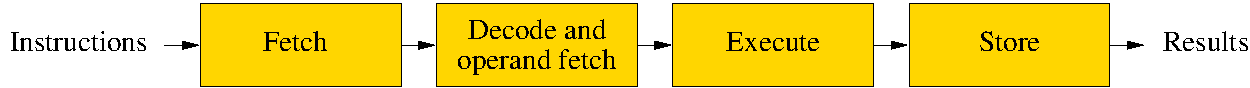
\includegraphics[scale=0.5]{pipeline-eps.pdf}
  }
  \caption{4-stage processor pipeline}
 \end{figure}

 \begin{itemize}
  \item ideally \( 1 \) instruction per pipeline per clock cycle
  \item need to keep the pipeline filled with instructions
  \item multiple next instructions possible after conditional branches
 \end{itemize}
\end{frame}

\begin{frame}
 \frametitle{CPU - Branching}
 \begin{itemize}
  \item processor tries to predice target of a conditional jump instruction
   \begin{itemize}
    \item statically (e.g., always expect true)
    \item dynamically with branch-prediction buffer
   \end{itemize}
  \item if correct, no overhead
  \item otherwise
  \begin{enumerate}
   \item processor throws away results of incorrect branch
   \item clears pipeline
   \item starts executing instructions of correct branch
  \end{enumerate}
  \item overhead of incorrect predictions depends on pipeline length (up to \( 20 \) clock cycles)
 \end{itemize}
\end{frame}

\begin{frame}
 \frametitle{CPU - Branch-less Code}
 \begin{itemize}
  \item example \filename{sgn.c}
  \item advantages
  \begin{itemize}
   \item no branch prediction necessary
   \item frees slots in the branch-prediction buffer
   \item often allows use of mutiple pipelines in parallel
  \end{itemize}
  \item disadvantages
  \begin{itemize}
   \item might require more computation
   \item no expensive computation possible
  \end{itemize}
 \end{itemize}
\end{frame}

\begin{frame}
 \frametitle{CPU - Branch-less Code}
 \begin{itemize}
  \item compute results without conditional jumps
  \item use multiply \( * \) instead of logical and \( \&\& \)
   \begin{itemize}
    \item \( \&\& \) does not evaluate right-hand side if left-hand side is false
    \item requires a conditional jump
    \item \( * \) always evaluates both sides, hence no conditional jump
   \end{itemize}
  \item use add \( + \) instead of logical or \( \vert\vert \)
   \begin{itemize}
    \item same as for \( \&\& \)
   \end{itemize}
  \item negate twice to compute \( 0 \) or \( 1 \)
   \begin{itemize}
    \item first negation maps \( 0 \) to \( 1 \), and any other value to 0
    \item second negation maps \( 1 \) back to \( 0 \), and \( 0 \) to \( 1 \)
   \end{itemize}
  \item do expensive computations beforehand, only use results
  \item use look-up tables for complex mappings
  \item \webpage{Bit Twiddling Hacks}{http://graphics.stanford.edu/~seander/bithacks.html}
 \end{itemize}
\end{frame}

\begin{frame}
 \frametitle{Memory - Look-up Tables}
 \begin{itemize}
  \item example \filename{lut.c}
  \item advantages
  \begin{itemize}
   \item map arbitrary input to arbitrary output
   \item predictable overhead
  \end{itemize}
  \item disadvantages
  \begin{itemize}
   \item additional overhead from memory access
  \end{itemize}
 \end{itemize}
\end{frame}

\begin{frame}
 \frametitle{Memory - Alignment}
 \begin{itemize}
  \item load instructions operate along word boundaries
 \end{itemize}

 \begin{figure}
  \centering {
   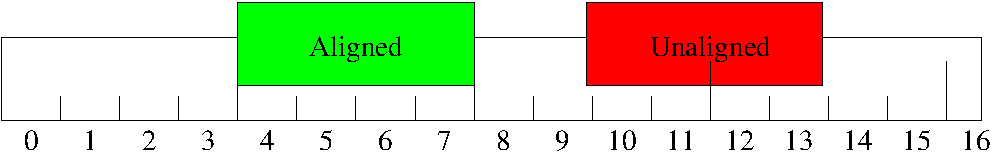
\includegraphics[scale=0.5]{maccess-eps.pdf}
  }
  \caption{Memory access}
 \end{figure}

 \begin{itemize}
  \item align data to word boundaries
  \begin{itemize}
   \item single load instruction
   \item ABI requires this
   \item gcc offers \sourcecode{\_\_attribute\_\_((align(\( n \))))}
  \end{itemize}
  \item can result in unused bytes within data structures
  \begin{itemize}
   \item example \filename{align.c}
   \item arrange structure fields according to alignment
   \item use \program{pahole} for optimizing data structures
  \end{itemize}
 \end{itemize}
\end{frame}

\begin{frame}
 \frametitle{Memory - Caches}
 \begin{itemize}
  \item processor fetches whole cache lines (\( 32 \), \( 64 \) Byte) at once
  \item align larger data structures to cache-line boundary
  \item first-used data should go at the beginning of cache line
  \item keep related data on the same cache line
  \item use data types with minimum size
  \item use individual bits
 \end{itemize}
\end{frame}

\begin{frame}
 \frametitle{Memory - False Sharing}
 \begin{itemize}
  \item two global variables with unrelated data might be located on the same cache line
  \item processor fetches whole cache lines at once
  \item unmodified cache lines are \binarycode{shared} by all processors
  \item writing to a cache line marks it as \binarycode{dirty}
  \item affects all contained values
  \item other processors will update their cache line from the modified copy even if they don't operate on the modified value
  \item known as \textit{False Sharing}
  \item try to put unrelated global data onto separate cache lines
 \end{itemize}
\end{frame}

\begin{frame}
 \frametitle{Memory - Cache Line Bouncing}
 \begin{itemize}
  \item processors use shared variables for communication with each other
   \begin{itemize}
    \item data exchange
    \item syncronization
   \end{itemize}
  \item write operations invalidate cache lines
  \item read operations need to fetch cache lines
  \item known as \textit{Cache Line Bouncing}
  \item can be avoided by good concurrency control
  \item \paperurl{U. Drepper}{What Every Programmer Should Know About Memory}{http://www.akkadia.org/drepper/cpumemory.pdf}
 \end{itemize}
\end{frame}

\begin{frame}
 \frametitle{Concurrency Control}
 \begin{itemize}
  \item mechanism of protecting concurrent access to shared resources against each other
  \item aka. locks vs. atomic ops
 \end{itemize}
\end{frame}

\begin{frame}
 \frametitle{Concurrency Control - Atomic Ops}
 \begin{itemize}
  \item atomic operations modify single values
  \item advantages
   \begin{itemize}
    \item good if lock contention is low
    \item no dead locks
   \end{itemize}
  \item disadvantages
   \begin{itemize}
    \item more overhead than non-atomic operations, because of bus lock
    \item no progress guaranteed (known as \textit{live lock})
   \end{itemize}
 \end{itemize}
\end{frame}

\begin{frame}
 \frametitle{Concurrency Control - Locking}
 \begin{itemize}
  \item works on arbitrary data
  \item advantages
   \begin{itemize}
    \item good if lock contention is high
    \item operating-system scheduler can guarantee fairness
   \end{itemize}
  \item disadvantages
   \begin{itemize}
    \item more initial overhead because of system-call
    \item dead locks possible
   \end{itemize}
  \item increase lock granularity if contention is high
 \end{itemize}
\end{frame}

\begin{frame}
 \frametitle{Tools}
 \begin{description}
  \item[\program{readelf}] information about ELF binaries
  \item[\program{perf}] system-wide profiling for Linux
  \item[\program{oprofile}] alternative to \program{perf}
  \item[\program{pahole}] layout of data structures in memory
 \end{description}
\end{frame}
